\documentclass[11pt,a4paper]{article}
\usepackage{hyperref}
\usepackage{emnlp2018}
\usepackage{times}
\usepackage{latexsym}
\usepackage{graphicx}
\usepackage{array}
\usepackage{float}
\usepackage{amsmath}

\usepackage{url}

\aclfinalcopy % Uncomment this line for the final submission

%\setlength\titlebox{5cm}
% You can expand the titlebox if you need extra space
% to show all the authors. Please do not make the titlebox
% smaller than 5cm (the original size); we will check this
% in the camera-ready version and ask you to change it back.

\newcommand\BibTeX{B{\sc ib}\TeX}
\newcommand\confname{EMNLP 2018}
\newcommand\conforg{SIGDAT}


\title{Making Chatbots Better by Training on Less Data}

\author{Richard Krisztian Csaky \\
  Department of Automation \\ and Applied Informatics \\
  Budapest University \\ of Technology and Economics \\
  {\tt ricsinaruto@hotmail.com} \\\And
  Gabor Recski \\
  Department of Automation \\ and Applied Informatics \\
  Budapest University \\ of Technology and Economics \\
  {\tt recski.gabor@aut.bme.hu} \\}

\date{\today}

\begin{document}
\maketitle
\begin{abstract}
% max. 200 words
    Current conversational models lack diversity and generate boring
responses to open-ended utterances \cite{Li:2015c,Wei:2017, Shao:2017b}.
    {\it Priors} provide additional information to dialogue models to
    aid response generation, but annotating a dataset with priors such
as persona \cite{Li:2016a}, emotion
\cite{Zhou:2017}, or topic \cite{Xing:2017}, is expensive and such
annotations are rarely available. We present a method for improving
    chatbots' responses to open-ended utterances by removing those
    utterances from
    training data using a simple entropy-based approach that
    does not require human supervision. We show that training
    on this filtered dataset results in better conversational quality as
    chatbots learn to output better and more diverse responses to these
    utterances.
\end{abstract}

\section{Introduction}
Current open-domain neural conversational models (NCM) are trained on
pairs of source and target utterances in an effort to maximize
the likelihood of each target given the source
\cite{Vinyals:2015d}. However, real-world conversations are much more complex,
and a plethora of suitable targets (responses) can exist to a given input.
We
remedy this issue by excluding from the training set inputs which are 
the ``most open-ended'', determined by calculating the entropy of the
distribution over target utterances.
We show that dialogue models
can be improved by using this simple filtering method, effectively training on
less data.

Previous approaches to the issues mentioned are discussed in
Section~\ref{sec:background}, and Section~\ref{sec:methods} describes our
method in detail.
Section~\ref{sec:experiments} presents an analysis of the filtered
dataset, dialogue systems trained on the new datasets are evaluated in
Section~\ref{sec:results}. Section~\ref{sec:conclusion} concludes and presents
future work.


\section{Background}
\label{sec:background}
Current open-domain NCMs are based on neural architectures developed
for machine translation (MT). Conversational data differs
greatly from MT data in that targets to the same source may vary not
only grammatically but also semantically
\cite{Wei:2017,Tandon:2017}; consider plausible replies to
the question: \textit{What did you do today?}. Dialogue datasets also
contain responses that appear after many different inputs, e.g. answers
such as \textit{yes}, \textit{no} and \textit{i don't
  know} appear after a large and diverse set of inputs.
Following the approach of modeling conversation as a sequence to sequence (\texttt{seq2seq})
\cite{Sutskever:2014} transduction of single dialogue turns, these
issues can be referred to as the
\textit{one-to-many}, and \textit{many-to-one} problem, respectively. Since
\texttt{seq2seq} architectures are inherently deterministic, meaning that once trained
they can't output different sequences to the same input sequence, they are not
suited to deal with the ambiguous nature of dialogues.
Related to these issues is the evaluation of open-domain
chatbots. Currently, there is no well-defined automatic evaluation method
(AVM) \cite{Liu:2016}, and many researchers resort to human evaluation
\cite{Vinyals:2015d, Serban:2017a, Ram:2018}. Some AVMs
that correlate with human judgement have been proposed recently
\cite{Li:2017a, Lowe:2017}, but they are harder to conduct than perplexity or BLEU \cite{Papineni:2002}.

The focus of this work is the \textit{one-to-many}, and \textit{many-to-one} problem,
previous approaches to which can be grouped into three
categories. First, the encoding procedure can be modified by feeding more
information into the model, like dialogue history \cite{Serban:2015}, persona
information \cite{Li:2016a,Joshi:2017,Zhang:2018}, mood/emotion category
\cite{Zhou:2017,Li:2017b}, topic category \cite{Xing:2017, Liu:2017}, etc. Second, some approaches augment the decoding process, with
e.g. latent variable sampling \cite{Serban:2017b,Zhao:2017} or
beam search \cite{Goyal:2017,Wiseman:2016,Shao:2017b}. Finally, directly
modifying the loss function \cite{Wiseman:2016} or training procedure of the
model, by using reinforcement \cite{Li:2016b,
  Serban:2017a,Li:2016c,Lipton:2017} or adversarial learning \cite{Li:2017a} are also
  among the solutions proposed.

\section{Methods}
\label{sec:methods}
% clustering and filtering

In this work the \textit{one-to-many}, \textit{many-to-one} issue is
approached from a different perspective: instead of adding more complexity, we
try simple data filtering methods to exclude source-target utterance pairs
that have high entropy, since we believe that these cause dialogue models to
output safe but boring responses. Entropy of utterances has also been used before for evaluation purposes \cite{Serban:2017b}. The entropy of a source/target utterance is
calculated based on the distribution of the target/source utterances that it
is paired with in the dataset. In essence, the learning task is formulated in
a way for which the maximizing likelihood approach is more suitable.
NCMs have been shown to produce better qualitative results after they overfit
the training data
\cite{Csaky:2017,Tandon:2017}. This also supports the claim that the loss
function is not capturing conversational goals, since a neural network model
should perform best when the validation loss is minimal. Our experiments
suggest that when training NCMs on our filtered datasets, validation loss
becomes a better indicator of the model's performance.

Of the 72 000 unique source utterances in the
DailyDialog dataset (see Section~\ref{sec:experiments} for details),
60 000 occur with only a single target. For these it seems
straightforward to maximize the conditional probability $P(T|S)$, $S$ and $T$ denoting
a specific source and target utterance.
However, in the case of sources that appear with multiple targets in the dataset,
models are forced to learn some ``average'' of
observed responses. This is the \textit{one-to-many} problem.
We can similarly formulate the \textit{many-to-one}
problem, where a diverse set of source utterances are observed with the
same target. This may be a less prominent issue in training NCMs,
since the probability of source utterances given some target
doesn't appear in standard loss functions (although it is used
in some special objective functions \cite{Li:2015c}). Still, we shall
experiment with excluding such targets (e.g. \textit{I don't know}),
since conversational models generate these quite frequently and they are
typically uninformative and unengaging (see Section~\ref{sec:eval} on
evaluation principles).

For each source utterance $s$ in the dataset we calculate the entropy
of the distribution $T|S=s$, i.e. given a dataset $D$ of source-target
pairs we define the
\textit{target entropy} of an utterance $s$ as 
\[ E_{\text{tgt}}(s, D) = - \sum_{(s, t_i)\in D} p(t_i|s)\log_2 p(t_i|s)
\]
Similarly, \textit{source entropy} of an utterance can be defined as
\[ E_{\text{src}}(t, D) = - \sum_{(s_i, t)\in D} p(s_i|t)\log_2 p(s_i|t)
\]
The probabilities are calculated based on the observed relative frequency of sentence pairs in the data. After calculating source and target entropies for each utterance in a
corpus, we filter the training data using one of 3 strategies. \textsc{target-based}, where pairs are filtered if the source utterance
has high target entropy. \textsc{source-based}, where
we filter based on the source entropy of the target utterance.
Finally, the \textsc{st-based} dataset is obtained by filtering pairs based on
both entropy values.

We also experimented with clustering utterances based on Jaccard similarity
between their bags of words (BoW), measuring the entropy of clusters
as opposed to individual utterances. Our intuition was that such a
cluster-based entropy may better reflect the semantic diversity of
all target/source utterances associated with some source/target. In
practice, however, this method proved inferior, bringing only noise to the simpler approach
in identifying the utterances that give rise to the most diverse sets of
responses. This may be due to the BoW model's inability to capture
semantic similarity. In Section~\ref{sec:conclusion} we briefly present our plans
for experimenting with different metrics in the future.


\section{Experiments}
\label{sec:experiments}
% actual filterings and trainings -> their results

\subsection{Dataset}
We use the DailyDialog
dataset\footnote{\url{http://yanran.li/dailydialog.html}} \cite{Li:2017b} in
our experiments. With 90 000 utterances in 13 000 dialogues, it is comparable in size
  with the Cornell Movie-Dialogs Corpus
\cite{Danescu:2011}, but contains real-world high quality dialogues, instead
of movie conversations, which are ``not truthful representations of real-life
conversations'' \cite{Danescu:2011}. The vocabulary was set to 16384, covering most of the words in the corpus (roughly 19000).

\subsection{Models}
For dialogue modeling we use \texttt{transformer} \cite{Vaswani:2017}, a novel
encoder-decoder architecture. Compared to the standard recurrent neural
network (RNN) based \texttt{seq2seq} models, it doesn't use recurrent connections
and relies only on attention mechanisms \cite{Bahdanau:2015}. Consequently, it can
be trained much faster, and using less memory (training the
\texttt{seq2seq}
model of \cite{Vinyals:2015d} was not possible with the 8GB of GPU
memory we had access to). We further justify the use of this model with the fact that it achieves
state-of-the-art performance in NMT. Since the original \texttt{seq2seq} model was
adopted from NMT \cite{Cho:2014} to dialogue modeling,
it is natural to do the same with the \texttt{transformer} architecture.
To justify its use for the dialogue task, we also train a
\texttt{seq2seq} model (of limited size) on the same dataset for comparison.
The \texttt{transformer} and \texttt{seq2seq} models contain 53M and 317M
parameters, respectively. They are both large compared to the dataset thus
they easily overfit it, as will be shown in Section~\ref{sec:results}.
In the case of the \texttt{transformer} model we also experimented with different
dropout \cite{Srivastava:2014a} values our findings will also be
presented in Section~\ref{sec:results}.

We trained randomly initialized word embeddings (of size 512) together with the model parameters. For the \texttt{transformer} model layer, attention, and relu dropout was set to 0.2, 0.1 and 0.1 respectively. At test time we used beam search with a beam size of 10 \cite{Graves:2012b}.

\subsection{Filtered data}
The 90 000 utterance pairs in the DailyDialog dataset contain about 72
000 unique utterances. We plot target entropies of source utterances in
Figure~\ref{fig:entropies}, ranked from lowest to highest entropy, not showing the majority of utterances which have 0 entropy (i.e. they do not appear with more than one target). Source entropies of target utterances are very similar. In the following
experiments we shall discard utterance pairs whose target and/or source entropy is greater
than 1. This affects 5.64\%, 6.98\% and 12.24\% of the data, for the \textsc{target-based}, \textsc{source-based} and \textsc{st-based} scenario, respectively.

\begin{figure}[!ht]
	\centering
	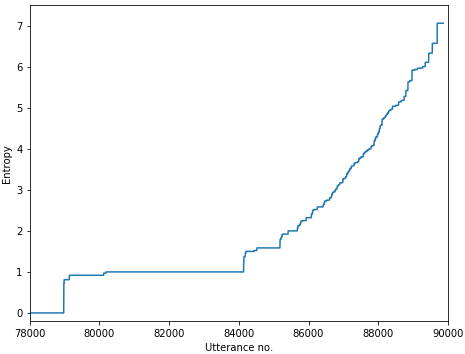
\includegraphics[width=0.47\textwidth]{pics/source_entropies.png}
	\caption{Source utterances by target entropy}
	\label{fig:entropies}
\end{figure}

Entropy is clearly proportional to utterance frequency
(Figure~\ref{fig:frequencies}), however we found that only 485 utterances overlap in the top 700 utterances (roughly what gets discarded) when ordered by both entropy and frequency, and those that are different in the frequency ordered list are long utterances, that we don't wish to filter out. Entropy offers a more fine-grained measure compared to frequency, and in the case of low frequency pairs, this is especially helpful. For example, all utterances that have a frequency of 3, are in the same category based on frequency, but their entropy can range from 0 to $\log_2 3\approx1.58$, which would be over our filtering threshold.



\begin{figure}[!ht]
	\centering
	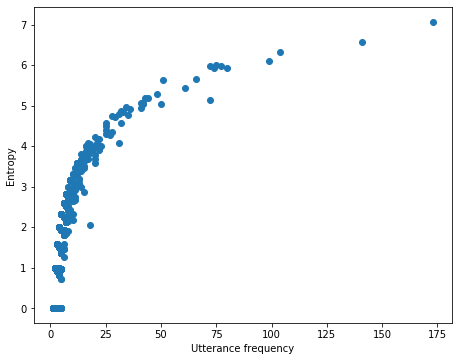
\includegraphics[width=0.47\textwidth]{pics/source_entropies_frequency.png}
	\caption{Target entropies of sources with respect to utterance frequency.}
	\label{fig:frequencies}
\end{figure}

After noticing that high-entropy utterances are relatively short, we
also examined the relationship between entropy and utterance length
(Figure~\ref{fig:length}). Given the relationship between frequency and
entropy it comes as no surprise that longer sentences have lower entropy,
although this effect is less pronounced in the range affected by filtering.

% and if they are unique then their
%entropy is 0, because the distribution consists of only 1 element.
\begin{figure}[!ht]
	\centering
	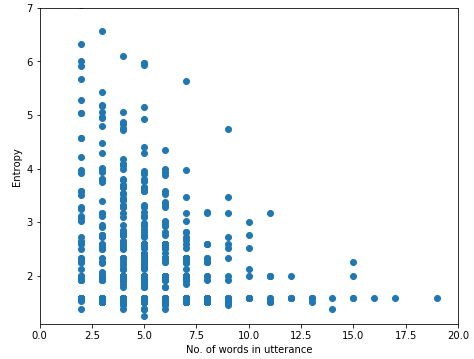
\includegraphics[width=0.47\textwidth]{pics/source_entropies_length.png}
	\caption{Target entropies of sources with respect to utterance length.}
	\label{fig:length}
\end{figure}

% ITT TARTOK (RG)
\section{Results}
\label{sec:results}
% compare \texttt{seq2seq} with transformer
% compare non-filtered and filtered trainings
% compare the different filtered trainings
% compare how overfitting affects the non-filtered and different filterings, for both models.
% also maybe show the top beams for the best filtered training and compare it with base
% Firstly a response has to be coherent, as much as a human response is. Only after it makes sense can we talk about whether it's boring or engaging
\subsection{Evaluation Principles}
\label{sec:eval}

Due to the limited scope of automatic evaluation
\cite{Liu:2016}, our claims are supported by both qualitative and quantitative evaluation of our models' outputs. We first summarize the principles used for
comparison, then present our findings. Because of space constraints we couldn't include the large samples of responses based on which we conducted the manual evaluation, but we invite readers to inspect the tables\footnote{\url{https://anonfile.com/54YeAbf6b6/tables.pdf}}.

We shall evaluate models based on answers they give to a list of input utterances.
When comparing responses given to the same question, we first consider
their \textit{coherence}, i.e. whether they could have been written by a
human speaker. Models that return coherent answers to an input
are further compared based on whether the answer is boring/generic (e.g.
\textit{I don't know}) or engaging/specific. 
Generic responses make sense in more dialogue histories, however because of this
they do not add new information to the
conversation. More engaging responses, i.e. those that can further a conversation,
are preferred, but only if they are coherent with the source utterance.
While these principles, and thus our judgements presented here, are quite subjective,
we believe that the differences observed between various trainings
are sufficiently pronounced, and our findings are also grounded by the quantitative analysis.

Four metrics are used to quantitatively evaluate our models in Section~\ref{ssec:qa}. In order to measure the information content of a models' responses, average utterance length \(|U|\), word entropy \(H_w\) and utterance entropy \(H_u\) is computed \cite{Serban:2017b}. The entropies are computed with respect to the maximum-likelihood unigram distribution of the training set. Thus: \(H_w=-\sum_{w\in{U}} p(w)\log(p(w))\), and \(H_u\) is simply the product of utterance length and word entropy. Additionally the average jaccard similarity \(J\) between source utterances and model responses is computed, measuring their coherence and relevance.  


\subsection{\texttt{seq2seq}, \texttt{transformer}, and overfitting}
\label{ssec:model_overfitting}

\begin{table}[t!]
	\small
	\begin{center}
		\begin{tabular}{p{1.2cm}p{1.1cm}p{1.8cm}p{0.4cm}p{1cm}}
			\textbf{Input} & \textbf{S2S} & \textbf{S2S-O} & \textbf{TRF} & \textbf{TRF-O} \\ \hline
			what is the color of water? & it's the best we can do it & leopard. it's famous for its quality only. & \textbf{it's red.} & \textbf{it's red.} \\ \hline 

			
		\end{tabular}
	\end{center}
	\caption{\label{table:ncm_test} Responses to an input utterance, by overfitted (O) and non-overfitted versions of the \texttt{seq2seq} (S2S) and \texttt{transformer} (TRF) models trained on unfiltered data. Best responses are boldfaced.}
\end{table}

We first compare overfitted and non-overfitted versions of the \texttt{seq2seq} (S2S) and
\texttt{transformer} (TRF) models trained on unfiltered data. Overfitted model versions,
are those that were trained further after the lowest value of validation loss
was reached, until training loss converges. We used a list of 34 general input utterances chosen from the ones used in \citet{Vinyals:2015d}, which we will call the NCM test inputs. We filtered this list by cutting well-known inputs to which each model learns to respond well (eg. \textit{Hello!}, \textit{How are you?}), and also removed inputs where any word was missing from the vocabulary.

For each question we determined the answers which we judged best, based on the
principles outlined at the beginning of this section. A representative row of the complete table can be seen in Table~\ref{table:ncm_test}. Generally,
the \texttt{transformer} performed better than the \texttt{seq2seq} model, achieving 11 best responses (among the 4 models), compared to only 7 for \texttt{seq2seq}. It managed to output colours when asked about the colour of objects, while the \texttt{seq2seq}'s replies were irrelevant.

Overfitted models performed at least as well (in human evaluation) as non-overfitted models,
strengthening the points raised in \citet{Csaky:2017, Tandon:2017}: the loss
function does not adequately represent the quality of a chatbot model. The overfitted \texttt{seq2seq} model achieved 9 best response (2 more than the non-overfitted version), and in the case of the \texttt{transformer} the overfitted version achieved 12 best responses. We noted that overfitted models tend to generate longer responses, which is generally good, but in some cases we obtain too specific
and probably memorized responses to unrelated inputs (eg. \textit{they have a
  really good dj and a good dance.}  to the input \textit{what is the purpose of
  dying}).

Since our models overfit quickly, we also experimented with dropout.
With a high dropout rate (0.5) we can essentially force the validation loss to stay at its minimum
for longer, before starting to overfit. However, the minimum does not
go lower compared to low dropout (0.2) trainings, and the replies were generally the
same even after training more with high dropout, further consolidating
the observation
that the validation loss minimum does not represent the best state of the model.

\subsection{High Entropy Inputs}
We evaluate the \texttt{transformer} model trained on unfiltered and filtered datasets (according to the 3 filtering types discussed in Section~\ref{sec:methods}) on the 45 highest entropy source utterances. These are the most challenging utterances (eg. \textit{yes; thank you; why?; sure; no; what's that?; here you are}), where dialogue models tend to fail, because of the high diversity observed in the dataset. The \textsc{target-based} filtering variant is excluded from this evaluation, because as we will see in Section~\ref{ssec:ncm_test_inputs} it performs poorly on the NCM test set, and also according to the automatic metrics (Section~\ref{ssec:qa}).

Counter-intuitively there is clear improvement in the performance on these utterances which the filtered models didn't see during training.
The \textsc{st-based} training gives the best response in 23 cases, while the unfiltered training only in 12 cases. Solely filtering the target side, gives slightly worse results, achieving only 11 best responses, however its responses can be often selected as the second-best after the \textsc{st-based}. A closer look at the \textsc{st-based} replies shows two main enhancements. First, the model was able to generate more diverse
responses, while also keeping them general enough (eg. \textit{I have a bad
	headache.}, or \textit{I'm glad to hear that.}), which is probably mostly due
the source-side filtering. Second, where the unfiltered model often choose to
output the same safe response (\textit{thank you.}), the
filtered model responds with engaging questions to
further the conversation. This is clearly due to the target side filtering,
since the model was forced to not learn to output generic responses. The conclusion is further reinforced by the \textsc{source-based} training, where the model answers with questions more frequently. However, the \textsc{source-based} training is still not diverse enough, combining the two methods seems the most advantageous. We also experimented with an overfitted variant of the \textsc{st-based} training, which performed a lot worse, and was too specific in many cases (giving the best response only in 7 cases). Overall it appears that with our filtered dataset the model performs better at the validation loss minimum.

\subsection{NCM test inputs}
\label{ssec:ncm_test_inputs}
We also evaluate the \texttt{transformer} model trained on unfiltered and filtered datasets on the NCM test inputs. The \textsc{st-based} and \textsc{source-based}
trainings are on par with the unfiltered training (15, 16, 15 best responses, respectively), followed by the \textsc{target-based} training (11 best responses). These results prove that the model is still capable to
output good responses to the general NCM test inputs, even when trained on the
filtered dataset. Filtering the source side alone gives worse results than filtering the target side alone, demonstrating that discarding generic responses adds more to conversational quality.

Finally, the overfitted version of the \textsc{st-based} training
performs slightly worse (getting best response in only 13 cases), somewhat alleviating the problems discussed in Section~\ref{ssec:model_overfitting}. As with the high entropy inputs, this indicates that filtering a dataset based on entropy, makes the learning problem more
aligned with the loss function.



\subsection{Quantitative Analysis}
\label{ssec:qa}

\begin{table}[t!]
	\small
	\begin{center}
		\begin{tabular}{lllll}
			
			\bf Unfiltered trainings & \(|U|\) & \(H_w\) & \(H_u\) & \(J\) \\ \hline
			
			\textsc{trf-base} & 4.93 & 0.493 & 2.43 & 0.091 \\
			\textsc{trf-base-o} & 9.82 & 0.797 & 7.83 & 0.099 \\
			\textsc{s2s-based} & 4.35 & 0.462 & 2.01 & 0.089 \\
			\textsc{s2s-base-o} & 7.09 & 0.628 & 4.45 & 0.098 \\ \hline
			\bf	Filtered trainings  &  &  &  &  \\ \hline
			
			\textsc{trf-st-based} & 6.31 & 0.586 & 3.70 & 0.099 \\
			\textsc{trf-st-based-o} & \bf10.42 & \bf0.838 & \bf8.73 & \bf0.101 \\
			\textsc{trf-target-based} & 5.25 & 0.525 & 2.76 & 0.096 \\
			\textsc{trf-source-based} & \textbf{\textit{6.81}} & \textbf{\textit{0.61}} & \textbf{\textit{4.15}} & \textbf{\textit{0.100}} \\ \hline
			
			\bf Targets & 14.10 & 1.031 & 14.54 & 0.105 \\ 
		\end{tabular}
	\end{center}
	\caption{\label{table:test_source} Quantitative metrics computed based on the test set. First, trainings which were trained on the normal (unfiltered) dataset are presented, and then trainings run on the filtered datasets. \textsc{trf} refers to the \texttt{transformer} model, and \textsc{s2s} refers to the \texttt{seq2seq} model. The type of filtering is also noted (\textsc{st-based}, \textsc{source-based}, \textsc{target-based}), and the \textsc{o} notation means that it is an overfitted version of the model. Results of best non-overfitted models are in italic boldface, while best results overall are noted by simple boldface.}
\end{table}

\begin{table}[t!]
	\small
	\begin{center}
		\begin{tabular}{lllllll}
			 & \multicolumn{2}{c}{\textsc{st-based}} & \multicolumn{2}{c}{\textsc{src-based}}  & \multicolumn{2}{c}{\textsc{tgt-based}} \\ \hline
			 & \textsc{base} & \textsc{filt} & \textsc{base} & \textsc{filt} & \textsc{base} & \textsc{filt} \\ \hline 
			\(|U|\) & 4.94 & \bf6.29 & 4.56 & \bf6.32 & 5.39 & \bf5.57 \\
			\(H_w\) & 0.512 & \bf0.598 & 0.481 & \bf0.604 & \bf0.551 & 0.541 \\
			\(H_u\) & 2.53 & \bf3.76 & 2.19 & \bf3.82 & 2.97 & \bf3.01 \\
			\(J\) & \bf0.121 & 0.099 & 0.115 & \bf0.119 & 0.130 & 0.130 \\
			
			
			
		\end{tabular}
	\end{center}
	\caption{\label{table:difference_source} Quantitative metrics computed from the responses of the base model and the 3 filtered trainings on 3 different test sets. The \textsc{st-based}, \textsc{source-based}, and \textsc{target-based} columns refer to test sets constructed by taking the difference between the unfiltered and the 3 filtered test sets respectively. \textsc{base} refers to the unfiltered \texttt{transformer} training, and \textsc{filt} refers to the 3 different types of filtered trainings.}
\end{table}

In Table~\ref{table:test_source} all metrics are computed based on responses given to a separate test set, containing 10\(\%\) of the utterances from DailyDialog. Looking only at the unfiltered trainings we can see that the \texttt{transformer} performed better than the \texttt{seq2seq} model across all metrics. In contrast to the manual evaluations however, on automatic metrics all examined overfitted models performed much better than their non-overfitted counterparts.

The results of the filtered trainings are also presented in Table~\ref{table:test_source}. It is clear that all types of filtering show significant improvement across all metrics. Interestingly, in contrast to the manual evaluations the \textsc{source-based} filtering achieves the best results, \textsc{st-based} being the second best, and aligned with the manual evaluations \textsc{target-based} is the last. Using \textsc{source-based} filtering alone, and thus filtering boring and generic responses is more important than \textsc{target-based} filtering, and combining the two types is not beneficial according to these metrics. Also, the overfitted version of the \textsc{st-based} training achieves the best performance, improving on the unfiltered training variant. Thus, while training on filtered datasets generally improves performance, a non-overfitted model still can't be competitive with an overfitted variant. However the performance gap between them gets somewhat smaller than in the case of unfiltered trainings. This also shows the limitation of these metrics that value diversity, since as seen in the manual evaluation, overfitted models tend to be too specific, by outputting learned responses.

We also constructed 3 smaller test sets, by taking the difference between the unfiltered test set and the filtered test sets (\textsc{st-based}, \textsc{source-based}, and \textsc{target-based}). With these test sets we want to show that the models trained on filtered data perform better even on the high entropy data that was filtered. Indeed in Table~\ref{table:difference_source} we can see that the filtered trainings generally performed better, \textsc{source-based} being the only test set and training that performed better than the model trained on unfiltered data across all metrics.


\section{Conclusion}
\label{sec:conclusion}
% + future work
We showed how with a simple entropy-based approach we can find generic and
safe sources/targets that usual dialogue models have problems with. We
compared the various trainings in an extensive qualitative and quantitative
evaluation. The unfiltered and the
filtered trainings were compared on two different objectively picked test sets, and on several automatic metrics used in the literature. We showed
how the model trained on the filtered dataset outputs more engaging and
interesting responses to inputs that it has never seen. Moreover, the \texttt{transformer} was shown to be at least as good for dialogue modelling as the \texttt{seq2seq}, and evaluating these models trained on unfiltered data at an overfitted point results in better conversational quality, while training on filtered data somewhat alleviates this issue.

% new for workshop
For future work we wish to try clustering methods, that
cluster based on ``semantic distance'', rather than syntactic
similarity. Sentence similarity is an active research area, and many approaches exist
such as word embedding averaging \cite{Arora:2016}, and RNN based methods \cite{Tai:2015}. We wish to use these sentence representations for clustering and filtering the dataset as described in Section~\ref{sec:methods}. Furthermore, we want to test our filtering approach together with
other approaches to the loss function problem discussed in
Section~\ref{sec:background}, like dialogue history.


\bibliography{ml}
\bibliographystyle{acl-natbib-nourl}
%\section*{Acknowledgments}


\end{document}

